\let\negmedspace\undefined
\let\negthickspace\undefined
\documentclass[journal]{IEEEtran}
\usepackage[a5paper, margin=10mm, onecolumn]{geometry}
\usepackage{lmodern} 
\usepackage{tfrupee} 
\setlength{\headheight}{1cm}
\setlength{\headsep}{0mm}   

\usepackage{gvv-book}
\usepackage{gvv}
\usepackage{cite}
\usepackage{amsmath,amssymb,amsfonts,amsthm}
\usepackage{algorithmic}
\usepackage{graphicx}
\usepackage{textcomp}
\usepackage{xcolor}
\usepackage{txfonts}
\usepackage{listings}
\usepackage{enumitem}
\usepackage{mathtools}
\usepackage{gensymb}
\usepackage{comment}
\usepackage[breaklinks=true]{hyperref}
\usepackage{tkz-euclide} 
\newcommand{\augvec}[3]{%
  \left(\begin{array}{*{#1}{c}|*{#2}{c}}
  #3
  \end{array}\right)}
\usepackage{listings}                             
\def\inputGnumericTable{}                                 
\usepackage[latin1]{inputenc}                                
\usepackage{color}                                            
\usepackage{array}                                            
\usepackage{longtable}                                       
\usepackage{calc}                                             
\usepackage{multirow}                                         
\usepackage{hhline}                                           
\usepackage{ifthen}                                           
\usepackage{lscape}
\usepackage{xparse}

\bibliographystyle{IEEEtran}

\title{4.11.36}
\author{EE25BTECH11059 - Vaishnavi Ramkrishna Anantheertha}

\begin{document}
\maketitle

\renewcommand{\thefigure}{\theenumi}
\renewcommand{\thetable}{\theenumi}

\numberwithin{equation}{enumi}
\numberwithin{figure}{enumi} 

\textbf{Question}:
Find the coordinates of the point where the line through the points $(3, -4, -5)$ and $(2, -3, 1)$ crosses the plane determined by the points $(1, 2, 3)$, $(4, 2, -3)$ and $(0, 4, 3)$.

\textbf{Solution }
\begin{table}[H]    
  \centering
  \begin{tabular}{|c|c|}
\hline
\textbf{Name} & \textbf{Value} \\ \hline
$\vec{A}$ & $\myvec{2 & 1 \\0 & 3}$ \\ \hline
\end{tabular}

  \caption{Variables Used}
  \label{tab:4.7.56}
\end{table}

Let eq of plane be
\begin{align}
    \vec{n^T}\vec{x}=1
\end{align}
As $\vec{P},\vec{Q},\vec{R}$ lie on the plane
\begin{align}
\vec{n^T}\vec{P}=1\\
\vec{n^T}\vec{Q}=1\\
\vec{n^T}\vec{R}=1\\
 \myvec{P^T 
        \\
        Q^T
        \\
        R^T}
\vec{n}
=
\myvec{1
       \\
       1
       \\
       1}
\end{align}
From eq $(0.2),(0.3),(0.4) and (0.5)$
\begin{align}
\augvec{3}{1}{
1 & 2 & 3 & 1 \\
4 & 2 & -3 & 1 \\
0 & 4 & 3 & 1}
&\xrightarrow{R_2 \to R_2 - 4R_1}
\augvec{3}{1}{
1 & 2 & 3 & 1 \\
0 & -6 & -15 & -3 \\
0 & 4 & 3 & 1} \\[6pt]
&\xrightarrow{R_2 \to -\tfrac{1}{3}R_2}
\augvec{3}{1}{
1 & 2 & 3 & 1 \\
0 & 2 & 5 & 1 \\
0 & 4 & 3 & 1} \\[6pt]
&\xrightarrow{R_3 \to R_3 - 2R_2}
\augvec{3}{1}{
1 & 2 & 3 & 1 \\
0 & 2 & 5 & 1 \\
0 & 0 & -7 & -1} \\[6pt]
&\xrightarrow{R_3 \to -\tfrac{1}{7}R_3}
\augvec{3}{1}{
1 & 2 & 3 & 1 \\
0 & 2 & 5 & 1 \\
0 & 0 & 1 & \tfrac{1}{7}} \\[6pt]
&\xrightarrow{R_2 \to R_2 - 5R_3}
\augvec{3}{1}{
1 & 2 & 3 & 1 \\
0 & 2 & 0 & \tfrac{2}{7} \\
0 & 0 & 1 & \tfrac{1}{7}} \\[6pt]
&\xrightarrow{R_2 \to \tfrac{1}{2}R_2}
\augvec{3}{1}{
1 & 2 & 3 & 1 \\
0 & 1 & 0 & \tfrac{1}{7} \\
0 & 0 & 1 & \tfrac{1}{7}} \\[6pt]
&\xrightarrow{R_1 \to R_1 - 3R_3}
\augvec{3}{1}{
1 & 2 & 0 & \tfrac{4}{7} \\
0 & 1 & 0 & \tfrac{1}{7} \\
0 & 0 & 1 & \tfrac{1}{7}} \\[6pt]
&\xrightarrow{R_1 \to R_1 - 2R_2}
\augvec{3}{1}{
1 & 0 & 0 & \tfrac{2}{7} \\
0 & 1 & 0 & \tfrac{1}{7} \\
0 & 0 & 1 & \tfrac{1}{7}
}
\end{align}


\begin{align}
\vec{n}=
\myvec{\frac{2}{7} 
       \\
       \frac{1}{7} 
       \\
       \frac{1}{7} 
}
\end{align}





hence eq of plane is
\begin{align}
 \myvec{\tfrac{2}{7} & \tfrac{1}{7} & \tfrac{1}{7}} 
 \vec{x}
 =1
\end{align}   


let a point on line $\vec{A}\vec{B}$ be 
\begin{align}
\vec{c}=k\vec{A}+(1-k)\vec{B}\\
\vec{n^T} 
(k\myvec{A}+(1-k)\myvec{B})
 =1\\
 \myvec{\frac{2}{7} & \frac{1}{7} & \frac{1}{7}}
 \myvec{2+k
               \\
              -3-k
              \\
              1-6k
 }=1\\
 4+2k-3-k+1-6k=7\\
2-5k=7\\
k=-1
\end{align}
The point $\vec{c}$ is
\begin{align}
    \vec{c}=\myvec{1
                   \\
                   -2
                   \\
                   7
             }
\end{align}
Refer to Figure

\begin{figure}[H]
\begin{center}
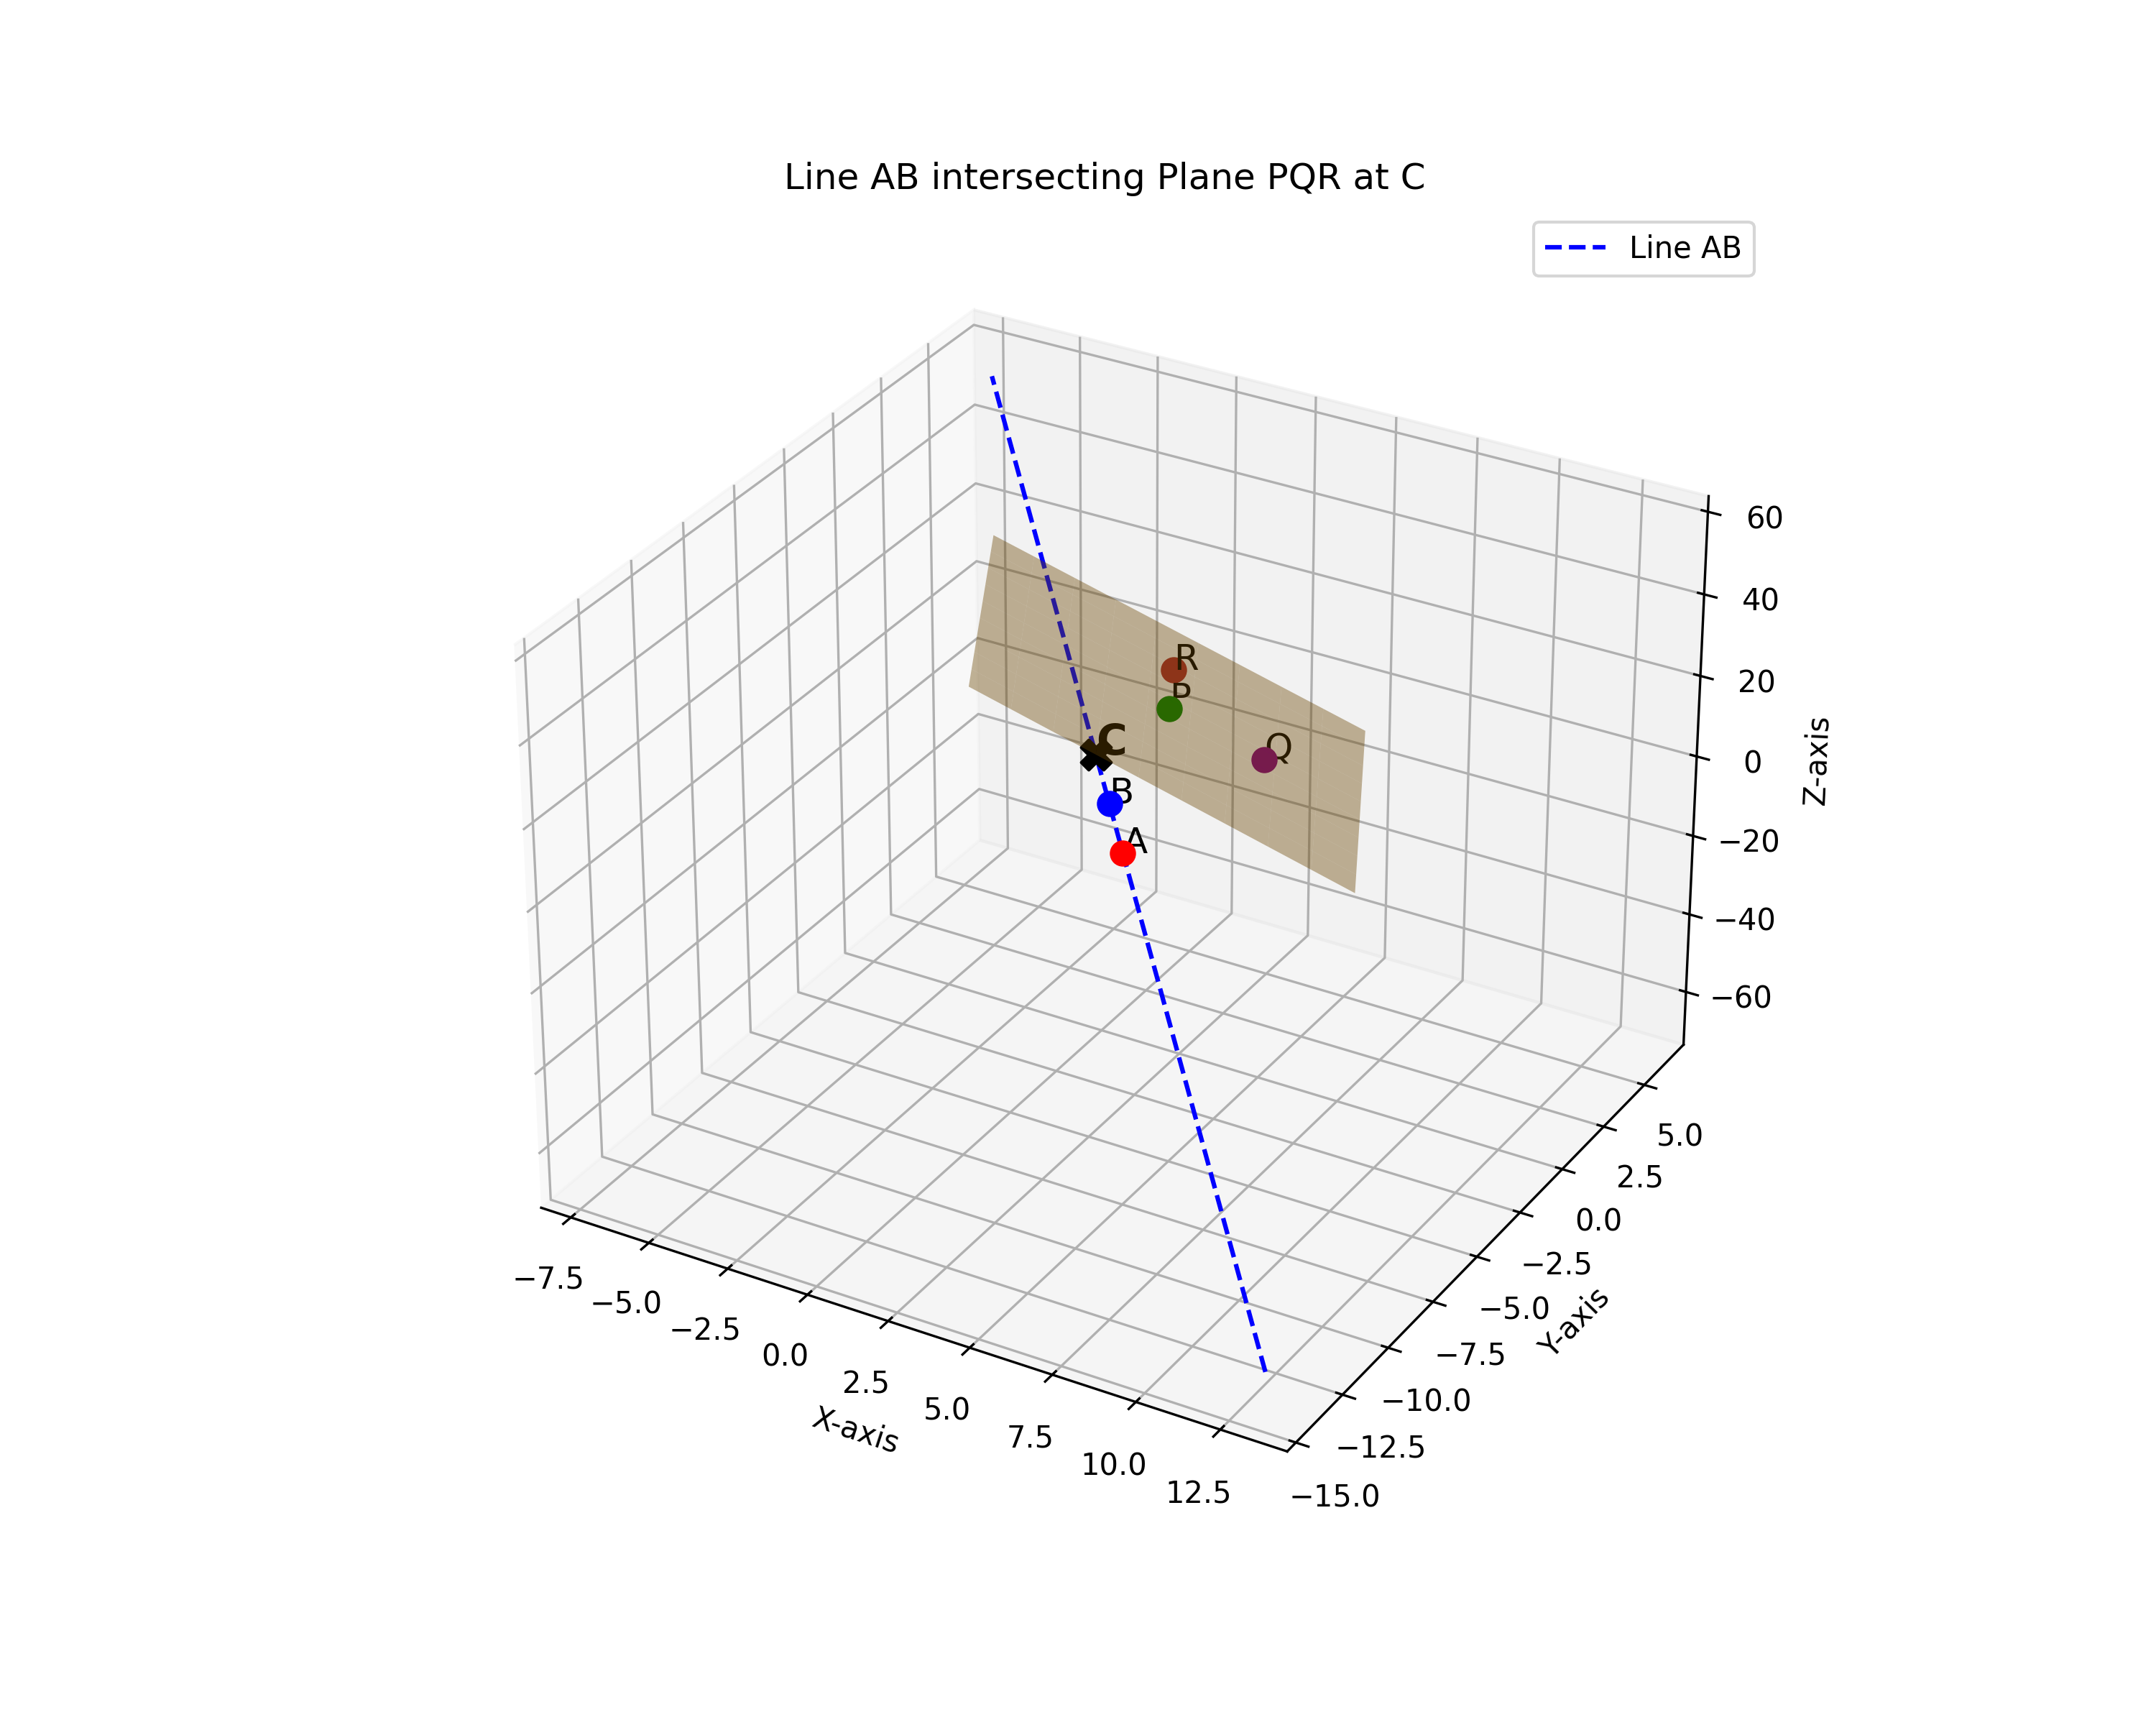
\includegraphics[width=0.6\columnwidth]{figs/graph8.png}
\end{center}
\caption{}
\label{fig:Fig}
\end{figure}
\end{document}